\documentclass[swe,12pt,nofont]{skrapport}
%% Packages (fold)
% Packages included by <skrapport>:
% polyglossia, microtype, icomma, amsmath,
% unicode-math, xunicode, fontspec
% graphics
\usepackage[usenames,dvipsnames]{xcolor}
\usepackage{graphicx}
\usepackage{tikz}
\usetikzlibrary{shadows}
% code
\usepackage{minted}
% improvement packages
\usepackage[hyperfootnotes=false,colorlinks=true,linkcolor=Red,urlcolor=Magenta]{hyperref}
\usepackage[swedish]{varioref}
\usepackage[para,perpage,ragged,bottom,stable]{footmisc}
\usepackage{enumitem}
\usepackage{fancyhdr}
\usepackage{booktabs}
% references
\usepackage[swedish]{chscite}
% other stuff
\usepackage{siunitx}
\usepackage{hologo}
\usepackage[safe,noenc]{tipa}
\usepackage[titles]{tocloft}
\usepackage{titlesec}
\usepackage[font=small,format=plain,labelfont=bf,textfont=it]{caption}
\usepackage{subfig}
\usepackage{cprotect}
%% (end)

%% FONT SELECTION (fold)
\defaultfontfeatures{%
	Numbers={Proportional,OldStyle},%
	Ligatures={Historic,Common,Required,Contextual},%
	Contextuals=Swash,%
	SmallCapsFeatures={Letters=SmallCaps,Scale=0.96,Weight=0.8},%
}
\setmainfont[Scale=1.1,SmallCapsFont={ArnhemSmallCaps}]{Baskerville}
\setsansfont[Scale=0.935]{Frutiger LT Std}
\setmonofont[Scale=0.935]{Prestige Elite Std}
\newfontfamily\titlefont[%
	Alternate=0,%
	%Ligatures={Rare,Historic,Common,Required,Contextual}%
]{Hoefler Text}
\newfontfamily\utffont{Times New Roman}% Change this?
\newfontfamily\tipafont{DejaVu Serif}
\setmathrm{Asana Math}
%\setmathsf{}
%\setmathtt{}
%\setboldmathrm{}
\makeatletter\newcommand\@titstyle{\titlefont}\makeatother
%% (end)

%% Hacks (fold)
\makeatletter
% Varioref seems broken with XeLaTeX
\def\reftextfaceafter {på \reftextvario{motstående}{nästa} sida}%
\def\reftextfacebefore{på \reftextvario{motstående}{föregående} sida}%
\def\reftextafter     {på \reftextvario{följande}{nästa} sida}%
\def\reftextbefore    {på föregående sida}%
\def\reftextcurrent   {på denna sida}%
\def\reftextfaraway#1{på sidan~\pageref{#1}}%
\def\reftextpagerange#1#2{på sidorna~\pageref{#1}–\pageref{#2}}%
\def\reftextlabelrange#1#2{\ref{#1} till~\ref{#2}}%
\DeclareRobustCommand\Vref{\@ifstar{\let\vref@space\relax\Vr@f}{\let\vref@space~\Vr@f}}
\DeclareRobustCommand\vref{\@ifstar{\let\vref@space\relax\vr@f}{\let\vref@space~\vr@f}}
% Twoside
\@twosidetrue
% Listings
\newcommand{\kodname}{Exempel}
\newcounter{kod}\renewcommand\thekod{\@arabic\c@kod}
\def\fps@kod{tb}
\def\ftype@kod{3}
\def\ext@kod{lok}
\def\fnum@kod{\kodname~\thekod}
\newenvironment{kod}{\@float{kod}}{\end@float}
\newenvironment{kod*}{\@dblfloat{kod}}{\end@dblfloat}
\newsubfloat{kod}
% Displaying one line of code
\newcommand\kodrad[2]{\hspace{1ex}\inputminted[firstline=#1,lastline=#1]{latex}{#2.tex}}
% Redefining sections to break page
\let\section@old=\section
\renewcommand\section{\@ifstar\my@section@star\my@section}
\newcommand\my@section[2][\@empty]{\cleardoublepage\vspace*{2\bigskipamount}\ifx\@empty#1\section@old{#2}\else\section@old[#1]{#2}\fi}
\newcommand\my@section@star[2][\@empty]{\cleardoublepage\vspace*{2\bigskipamount}\ifx\@empty#1\section@old*{#2}\else\section@old*[#1]{#2}\fi}
% Front/main/backmatter
\newcommand\frontmatter{%
  \cleardoublepage
  \pagenumbering{roman}}
\newcommand\mainmatter{%
  \cleardoublepage
  \pagenumbering{arabic}}
\newcommand\backmatter{%
  \cleardoublepage
}
% Maketitle without newpage
\newcommand\maketitlennp{\par%
  \begingroup
    \renewcommand\thefootnote{\@fnsymbol\c@footnote}%
    \def\@makefnmark{\rlap{\@textsuperscript{\normalfont\@thefnmark}}}%
    \long\def\@makefntext##1{\parindent 1em\noindent%
      \hb@xt@1.8em{\hss\@textsuperscript{\normalfont\@thefnmark}}##1}%
    \global\@topnum\z@
    \@maketitlennp
    \thispagestyle{empty}\@thanks
  \endgroup
  \setcounter{footnote}{0}
}
\def\@maketitlennp{%
  \null
  \begin{flushleft}%
\vspace{-\headsep}
    {\small%
      \if\@regarding\relax\else\@regarding{, }\fi%
      \@date\par%
    }%
    \vspace{1.5cm}%
    {\Huge\@titstyle\@title\par}%
    \vspace{.125cm}%
    {\Large\@titstyle\@author}%
    \vspace{.75cm}%
  \end{flushleft}%
  \par%
}
% Changes to titlepage environment (don't reset pagenumbering before)
\renewenvironment{titlepage}{\cleardoublepage}{\thispagestyle{skrapport@titlepage}\cleardoublepage\setcounter{page}\@ne}
% TexorPDF version of LaTeX and AmS logo
\let\@oldLaTeX\LaTeX
\def\LaTeX{\texorpdfstring{\@oldLaTeX}{LaTeX}}
\let\@oldAmS\AmS
\def\AmS{\texorpdfstring{\@oldAmS}{AMS}}
% File last modified
\def\parsedate #1:2#2#3#4#5#6#7#8#9\empty{\ifx{#2}{9}19\else20\fi#3#4/#5#6/#7#8}
\newcommand\moddate[1][\jobname.tex]{\expandafter\parsedate\pdffilemoddate{#1}\empty}
\makeatother
% (end)

%% Convenient definitions (fold)
\newcommand\PDF{\textsc{pdf}}							% PDF format
\newcommand\DVI{\textsc{dvi}}							% DVI format
\newcommand\EPS{\textsc{eps}}							% EPS format
\newcommand\UTF{\textsc{utf-8}}							% UTF-8 standard
\newcommand\cli[1]{\texttt{#1}}							% Command-line input
\newcommand\opt[1]{\texttt{\emph{#1}}}					% CLI option
\newcommand\pack[1]{\textsf{#1}}						% LaTeX package
\newcommand\pdfLaTeX{\hologo{pdfLaTeX}}					% pdfLaTeX logotype
\newcommand\BibTeX{\textsc{Bib}\TeX}					% BibTeX logotype
\newcommand\PGFTikZ{PGF/Ti\emph{k}Z}					% PGF/TikZ logotype
\newcommand\XeTeX{\hologo{XeTeX}}						% XeTeX logotype
\newcommand\LyX{L\!\raisebox{-.5ex}{Y}\!X}				% LyX logotype
\newcommand\eng[1]{(eng.~\emph{#1})}					% english translation
\newcommand\cmd[1]{\texttt{\textbackslash{}#1}}			% LaTeX command
\newcommand\env[1]{\texttt{#1}}							% LaTeX environment
\newminted{latex}{frame=single}							% LaTeX source code
% Front/back page color and graphics
\def\frontpagecolor{LimeGreen}
\newcommand\frontpagegraphic{\begin{tikzpicture}[remember picture,overlay]
	\coordinate [below=4.225cm] (midpoint)
					   at (current page.north);
	\node [anchor=north,fill=Black,opacity=0.25,
	minimum width=\paperwidth,
	minimum height=6cm] at (midpoint) {};
\end{tikzpicture}}
% Unit definitions
\DeclareSIUnit\point{pt}
%% (end)

%% Redefinitions of style (fold)
\setcounter{secnumdepth}{1}				% Section numbering depth
\setcounter{tocdepth}{2}				% Table of contents depth
\renewcommand{\cftsecfont}{\bfseries}	% Table of contents bf sections
\fancypagestyle{thefancy}{%
	\fancyhead{}
	\fancyfoot{}
	\fancyhead[LE,RO]{\thepage}
	\renewcommand{\headrulewidth}{0.1pt}
}
\headheight 15pt
\makeatletter
\renewcommand\thesection{\Roman{section}}
\titleformat{\section}[block]{\centering\Huge\@titstyle}{\makebox[\textwidth]{\fontsize{36pt}{36pt}\selectfont\centering\thesection}}{0pt}{\newline}[\bigskip]
% Holy shit, hacking my own class
% <FIXME> Buggigt utan stjärna på subsubsubsection. Varför?
\let\c@paragraph\relax\let\c@subparagraph\relax 
\let\paragraph\relax\let\subparagraph\relax
\newcommand\subsubsubsection{\@startsection{subsubsubsection}{4}{\z@}%
  {-2ex \@plus .5ex \@minus -.5ex}%
  {.125ex \@plus.125ex}%
  {\normalfont\large\@titstyle\itshape}}
\newcommand\paragraph{\@startsection{paragraph}{5}{\z@}%
  {1ex \@plus .25ex \@minus -.25ex}%
  {-1em}%
  {\normalfont\normalsize\bfseries}}
\newcommand\subparagraph{\@startsection{subparagraph}{6}{\parindent}%
  {1ex \@plus .25ex \@minus -.25ex}%
  {-1em}%
  {\normalfont\normalsize\itshape}}
\newlistentry[subsubsection]{subsubsubsection}{toc}{3}
\newlistentry[subsubsubsection]{paragraph}{toc}{4}
\newlistentry[paragraph]{subparagraph}{toc}{5}
\cftsetindents{subsubsubsection}{6.45em}{4.15em}
\cftsetindents{paragraph}{10.6em}{5.15em}
\cftsetindents{subparagraph}{15.75em}{6.15em}
\providecommand*{\toclevel@subsubsubsection}{4}
\providecommand*{\toclevel@paragraph}{5}
\providecommand*{\toclevel@subparagraph}{6}
\renewcommand\thesubsubsubsection{\thesubsubsection.\@arabic\c@subsubsubsection}
\renewcommand\theparagraph{\thesubsubsubsection.\@arabic\c@paragraph}
\renewcommand\thesubparagraph{\theparagraph.\@arabic\c@subparagraph}
\makeatother
%% (end)

%% METADATA (fold)
\title{Att \TeX{}a: en praktisk guide}
\author{Simon Sigurdhsson}
\regarding{Nybörjarguide i \LaTeX}
\date{första upplagan.}
%% (end)

\begin{document}
	\pagestyle{empty}
	\pagenumbering{Alph}
	
	{ % EXTERNAL FRONT PAGE (fold)
		\pagecolor{\frontpagecolor}
		\color{White}
		\frontpagegraphic
		\maketitlennp		
		\normalcolor
		\newpage
		\pagecolor{White}
	} % (end)
	\cleardoublepage
	
	\begin{titlepage} % INTERNAL TITLE PAGE (fold)
		\license{%Senast uppdaterad \moddate{}.\\
		Licenserad under Creative Commons By-Nc-Nd-2.5.\\
		\url{http://creativecommons.org/licenses/by-nc-nd/2.5/se/}\\
		För användning utanför licensen, kontakta författaren.}
		\maketitle
		\begin{abstract}
			En inkomplett guide till att skriva och typsätta \LaTeX-dokument riktad
			till studenter på Chalmers Tekniska Högskola, specifikt programmen
			Teknisk Matematik och Teknisk Fysik.
			Inspiration har tagits från bland annat \citeasnoun{Schultz05} och
			\citeasnoun{Voss10}, men främst från \citeasnoun{Oetiker11}.
		\end{abstract}
	\end{titlepage} % (end)
	\cleardoublepage
	
	\frontmatter
	\pagestyle{thefancy}
	\tableofcontents
	\cleardoublepage
	
	\mainmatter
	%% INLEDNING (fold)
	\section*{Inledning}
	\addcontentsline{toc}{section}{\hspace{1.3em}Inledning}
	Att publicera något, oavsett om det är långa böcker eller korta artiklar,
	är inte helt enkelt. Förr, innan det fanns en dator i varje hem och innan
	programvaror som Microsoft Word och OpenOffice blev tillgängliga för var
	man så var publicering något komplext, något som utfördes av många olika
	personer. Arbetet delades upp i olika bitar och en expert inom varje
	område fick sköta den biten; författande, typsättning, design och så
	vidare.
	
	Moderna programvaror (ordbehandlare, främst) fungerar på ett helt annat
	sätt. De ger all makt till författaren, som givetvis inte alltid är
	särskilt bra på det där med typsättning eller design. Som en konsekvens
	blir typsättningen av dokument inte alltid bra — användarna är under
	illusionen att ett estetiskt tilltalande dokument även är ett bra dokument
	rent typografiskt. Så är givetvis inte fallet.
	
	För att få snygga dokument måste man återskapa den gamla ordningen då
	varje uppgift löstes av någon som var bra på det. En författare ska inte
	behöva berätta \emph{hur} saker ska se ut — det ska designern göra —
	författaren ska bara berätta \emph{vad} saker är\footnote{Detta är inte
	helt olikt den uppdelning som görs mellan HTML och CSS.}. \LaTeX{} låter
	dig som författare göra just detta.
	
	\subsection*{Vad är \LaTeX{}?}
	\addcontentsline{toc}{subsection}{Vad är \LaTeX{}?}
	\LaTeX{} (uttalas \textipa{\tipafont[\textprimstress lA:tEx]}) är i princip en
	påbyggnad till \TeX{}, ett typsättningssystem. Man kan även se det som att
	\LaTeX{} är designern, och \TeX{} är typsättaren. \LaTeX{} berättar i
	någon mening för \TeX{} hur den tror att du vill ha ditt dokument (utifrån
	dokumentklassen samt den kod du skriver) och låter sedan \TeX{} typsätta
	detta för att skapa ett ”tryckt” dokument.
	
	Men \LaTeX{} är inte bara ett typsättningssystem; både språket dokumenten
	skrivs i och den kompilator som omvandlar dokumenten till \DVI-filer
	kallas också \LaTeX{} (men just kompilatorn brukar benämnas \cli{latex},
	eftersom det är så den körs från terminalen). Det finns även modernare
	versioner av \LaTeX{}-kompilatorn, till exempel \pdfLaTeX{} som skapar
	\PDF-dokument
	 direkt (så att man slipper konvertera dem med \cli{dvipdf}) och
	\XeTeX{}, som baseras helt på \textsc{Unicode} och har bättre stöd för
	diverse typsnitt.
	
	\subsection*{Varför \LaTeX?}
	\addcontentsline{toc}{subsection}{Varför \LaTeX{}?}
	Fördelen med \LaTeX{} är då att författaren endast behöver lära sig några
	enkla kommandon — sådana som gör texten kursiv eller infogar en figur
	— men att dokumentet ändå håller mycket hög standard, precis som om
	det typsatts av en riktig typsättare.
	
	Eftersom språket man skriver dokument i uppmanar till struktur och ordning
	blir det dessutom lättare att skriva strukturerade texter. Även om saker
	som finns i en vanlig ordbehandlare (stavningskontroll, till exempel) saknas i
	själva språket så kan (och bör) dessa tillhandahållas av externa program,
	vilket gör att \LaTeX{} kan koncentreras på att vara bra på \emph{en} sak:
	att typsätta dokument. Saker som är komplicerade eller omöjliga att göra
	i en vanlig ordbehandlare, till exempel korsreferenser, figurer, tabeller,
	fotnoter, referenslistor och dylikt är oerhört enkla att göra i \LaTeX{}
	och oftast fullt automatiserade.
	
	Dessutom har \LaTeX{} traditionellt använts av akademiker eftersom det gör 
	typsättning av just matematik och fysik både enkel och visuellt attraktiv. 
	
	\subsection*{I denna introduktion}
	\addcontentsline{toc}{subsection}{I denna introduktion}
	Den här korta introduktionen kommer att visa dig hur man på ett enkelt
	sätt typsätter dokument med \LaTeX{} i vanliga tillämpningar.
	Dessutom kommer den framåt slutet peka på specifika paket eller
	resurser som kan vara användbara för mer avancerade fall.
	
	Efter att ha läst den här introduktionen bör läsaren kunna skriva
	dokument och rapporter utan problem. Det är dock inte tänkt att denna
	introduktion ska vara en fullgod referens till \LaTeX; för detta
	rekommenderas istället \citeasnoun{Lamport94} och
	\citeasnoun{Mittelbach04}.
	
	Introduktionen innehåller följande delar:
	\begin{description}
		\item[{Del \ref{sec:1}, \hyperref[sec:1]{Grundläggande begrepp}}]
		beskriver den grundläggande strukturen hos \LaTeX-dokument och hur det
		språk dokumenten skrivs i fungerar i korta drag. Efter denna del bör
		du veta på ett ungefär hur \LaTeX{} fungerar.
		
		\item[{Del \ref{sec:2}, \hyperref[sec:2]{Typsättning med \pdfLaTeX}}]
		beskriver i detalj hur man skriver ett vanligt
		\LaTeX-dokument, och förklarar några av de viktigaste miljöerna
		och kommandona som används. Efter denna del bör du kunna skriva enkla
		dokument med \LaTeX.
		
		\item[{Del \ref{sec:3}, \hyperref[sec:3]{Matematik med \LaTeX{} och 
		\AmS}}]
		beskriver hur man på bästa sätt använder \LaTeX{} tillsammans med
		\AmS-paketen för att typsätta det \LaTeX{} typsätter bäst; matematik,
		och går även kort in på hur man typsätter en del fysik med paketet
		\pack{siunitx}.
		
		\item[{Del \ref{sec:4}, \hyperref[sec:4]{Grafik med \LaTeX}}]
		beskriver hur man inkluderar grafik i \LaTeX{} med paketet
		\pack{graphicx}, och visar några korta exempel på hur man kan rita
		direkt i \LaTeX{} med \PGFTikZ{}. Efter den här och föregående del bör
		du kunna skriva fullständiga rapporter med \LaTeX.
		
		\item[{Del \ref{sec:5}, \hyperref[sec:5]{Referenser med \BibTeX}}]
		beskriver hur du använder \BibTeX{} för att hålla koll på och använda
		referenser i \LaTeX. Beskriver i korthet paketet \pack{chscite} som
		hjälper dig att typsätta referenser på det sätt Chalmers bibliotek
		rekommenderar. Efter denna delen bör du kunna skriva långa arbeten
		(till exempel kandidatrapporter) i \LaTeX.
		
		\item[{Del \ref{sec:6}, \hyperref[sec:6]{Vidare läsning}}]
		tipsar om andra resurser, paket, dokumentklasser och rekommendationer
		som kan vara av nytta när du skriver långa (eller korta) rapporter.
		Kan vara en språngbräda om du vill göra något som inte förklaras i
		resten av introduktionen.
		
		\item[Appendix \ref{app:1}, {\hyperref[app:1]{En enkel mall}}]
		innehåller en mall du med fördel kan basera dina framtida 
		\LaTeX{}-dokument
		på. Den är fullt kommenterad och motiverar de paket som inkluderas och
		kommandon som definieras.
	\end{description}
	
	Det är viktigt att läsa delarna i rätt ordning; varje del bygger på de
	föregående, och de är ju trots allt inte särskilt långa. Se till att
	studera och förstå de exempel som presenteras, och lek gärna lite själv
	om du inte riktigt förstår. Det finns inget bättre sätt att lära sig än
	att vara nyfiken!
	
	\LaTeX{} finns till många plattformar, och finns installerat på Chalmers
	Linuxdatorer. Vill du installera \LaTeX{} på din egen dator finns det
	sannolikt i din pakethanterare (om du använder Linux), alternativt i form
	av \TeX{} Live\footnote{\url{http://www.tug.org/texlive/}}. Använder du
	Mac OS~X finns det istället
	Mac\TeX\footnote{\url{http://www.tug.org/mactex/}}, och till Windows finns
	MiK\TeX\footnote{\url{http://miktex.org/}}. Den här introduktionen kan
	tyvärr inte ge fullständiga instruktioner för att installera dessa paket
	(det är inte introduktionens syfte);
	konsultera istället respektive pakets dokumentation.
	
	Under introduktionens gång kommer det refereras till så kallade
	\emph{paket}, som används för att utöka \LaTeX{} med intressanta (och
	ibland nödvändiga) funktioner. Dessa paket kommer oftast att beskrivas
	lite kort, men vill man se fullständig dokumentation för varje paket
	kan man leta på \emph{the Comprehensive \TeX{} Archive Network}
	(CTAN)\footnote{\url{http://www.ctan.org/}}. Det lättaste sättet att hitta
	paket på CTAN är att använda dess
	sökfunktion\footnote{\url{http://www.ctan.org/search/}}.
	%% (end)
	 
	%% GRUNDLÄGGANDE BEGREPP (fold)
	\section{Grundläggande begrepp}\label{sec:1}
	Introduktionen har förklarat lite kort vad \TeX/\LaTeX{} är och varför du
	bör använda systemet för att typsätta dina rapporter, artiklar och böcker.
	Denna del kommer att inleda din \TeX-bana genom att lite kort förklara hur
	ett \LaTeX-dokument är uppbyggt, några viktiga begrepp samt hur
	\LaTeX-kompilatorn (i det här fallet \cli{pdflatex}) fungerar.
	
	\subsection{\LaTeX-dokument}
	De dokument \LaTeX{} läser in är enkla textfiler, oftast med filändelsen
	\cli{.tex}. Dessa kan skapas med vilken textredigerare som helst (till
	exempel Emacs på Linux-system), men det rekommenderas att man använder
	en textredigerare med syntaxfärgning (då det underlättar felsökande) och
	stavningskontroll. Oftast sparar man filen med teckenkodningen \UTF{} 
	(detta gör de flesta moderna textredigerare), men det finns en risk att
	filerna sparas med teckenkodningen \textsc{iso-8559-1}\footnote{Det finns 
	även andra teckenkodningar som kan dyka upp; Windows-1252 är en sådan.}, 
	och då måste man ha koll på detta eftersom man måste berätta för \LaTeX{}
	hur filen ska läsas in.
	
	\subsubsection{Tomrum}
	Tomrumstecken, det vill säga mellanslag, tabbar och liknande behandlas
	alla som ”tomrum” av \LaTeX{}. Flera sådana tecken i rad tolkas som ett
	enda tomrum, vilket gör att man kan ex. indentera textstycken i sin
	\LaTeX-fil utan att detta påverkar resultatet. Tomrum i början av en rad
	ignoreras generellt sett, och ett enkelt nyradstecken tolkas också som
	tomrum.
	
	Två nyradstecken på rad (det vill säga en tom rad mellan två textrader) tolkas som
	styckesindelning, och flera tomma rader efter varandra tolkas som en enda
	tom rad. Detta gör att \LaTeX{}-filerna blir mycket enkla att både skriva
	och läsa, även om man inte är en särskilt bevandrad \TeX{}niker.
	
	\subsubsection{Specialtecken}
	Vissa tecken är speciella för \LaTeX{}. Dessa används i \LaTeX{} och dess
	kommandon, och om man använder dem direkt i sin text så kan vad som helst
	hända. Vanligtvis slutar det bara med att tecknet inte syns, men det kan
	potentiellt göra att ditt dokument inte ens kompilerar. Specialtecknen
	är inte särskilt många:
	\mint{latex}|# ^ & _ { } ~ \ % $|
	
	För att använda dem måste man lägga till ett (bakvänt) snedstreck,
	\cmd{}, innan tecknet man vill använda (dock ej innan
	\cmd{} självt, eftersom \LaTeX{} tolkar
	\cmd{\textbackslash} som att man vill tvinga fram en
	radbrytning — vill man ha ett \cmd{} använder man istället
	\cmd{textbackslash}).
	När det gäller \verb|^| och \verb|~| måste man
	dessutom lägga till måsvingar efteråt, eftersom dessa kan användas för att
	modifiera vokaler. Tecknen måste alltså skrivas på följande sätt:
	\mint{latex}|\# \^{} \& \_ \{ \} \~{} \textbackslash \% \$|
	
	\subsubsection{\LaTeX-kommandon}
	För att säga åt \LaTeX{} vad som ska göras används kommandon. De flesta
	kommandona i \LaTeX{} följer några enkla regler:
	\begin{itemize}
		\item De börjar med ett bakvänd snedstreck (\cmd{}) och följs av sitt
		namn, som bara får innehålla bokstäver%
		\footnote{Det finns även ett antal kommandon som består av \cmd{} och
		exakt en icke-bokstav, till exempel \cmd{\&}.}.
		Kommandon avslutas av ett
		mellanslag, en siffra eller annan godtycklig ”icke-bokstav”.
		
		\item De är skriftlägeskänsliga (\cmd{Kommando} är inte samma sak som
		\cmd{kommando}).
		
		\item Vissa kommandon har även en ”stjärnvariant”, då en stjärna
		(\texttt{*}) läggs till på slutet av kommandonamnet.
	\end{itemize}
	
	\LaTeX{} ignorerar tomrum efter ett kommando. Det är därför nödvändigt, om
	man vill ha ett mellanslag efter ett kommando, att lägga till antingen en
	tom parameter \texttt{\{\}} och ett mellanslag eller ett speciellt
	mellanslagskommando (till exempel \texttt{\~{}}) mellan
	kommandot och nästa ord. Detta stoppar \LaTeX{} från att äta upp allt
	tomrum efter kommandot.
	
	Vissa kommandon kräver en obligatorisk och/eller frivillig parameter som
	på ett eller annat sätt bestämmer hur kommandot beter sig. Den generella
	strukturen hos ett kommando, med dessa parametrar, är relativt enkel:
	\mint{latex}|\kommando[frivillig parameter]{obligatorisk parameter}|
	
	Finns det ingen obligatorisk parameter, eller om den frivilliga parametern
	inte används, kan hela biten inklusive hakparantes/måsvinge helt
	utelämnas.
	
	\subsubsection{Kommentarer}
	Ibland kan det vara bra att kommentera bort (alltså~säga åt \LaTeX{} att
	ignorera) vissa bitar av till dokument. Det kan vara för att förklara
	olika kommandon eller definitioner, eller för att ta bort ett stycke man
	inte är helt säker på. Detta görs med procenttecknet; när \LaTeX{} stöter
	på ett sådant (såvida det inte sitter ett \cmd{} före) så ignorerar den
	hela resten av den raden i \TeX{}-filen:
	\mint{latex}|Lite text\ldots{} % ...och en kommentar|
	
	\subsubsection{Grundläggande struktur}
	När du nu vet hur \LaTeX{} tolkar tomrum, vad ett kommando är och hur du
	kommenterar delar av dina filer är det dags att förklara lite närmre hur
	en typisk \LaTeX{}-fil ser ut. Kompilatorn förväntar sig en viss struktur,
	till exempel så måste varje dokument inledas med kommandot
	\mint{latex}|\documentclass{...}|
	som berättar för \LaTeX{} vilken dokumentstil du vill använda (det finns
	ett antal olika, för till exempel rapporter, böcker eller brev).
	
	Därefter bör man köra de kommandon som påverkar hela dokumentet, till
	exempel så kan man ladda in extra paket eller definiera nya kommandon.
	Paket laddar man in med kommandot \cmd{usepackage}:
	\mint{latex}|\usepackage{...}|
	
	Båda dessa kommandon tar en obligatorisk parameter (namnet på 
	stilen/paketet) och en frivillig parameter som används för att skicka
	inställningar till stilen eller paketet som laddas in — en närmare
	förklaring av båda dessa kommandon finns \vpageref{sec:1:layout}.
	
	När allt förarbete är gjort kan man inleda dokumentet. Först berättar man
	för \LaTeX{} att innehållet börjar med hjälp av kommandot
	\mint{latex}|\begin{document}|
	och därefter följer dokumentets innehåll. När allt innehåll är slut
	avslutar man dokumentet med det snarlika kommandot
	\mint{latex}|\end{document}|
	som säger åt \LaTeX{} att det inte finns något mer som ska typsättas.
	
	\subsection{Dokumentets layout}\label{sec:1:layout}
	\LaTeX{} är inte helt oflexibelt, och man kan med hjälp av olika kommandon
	i inledningen till dokumentet ändra både utseendet och beteendet av
	dokumentet. Utseendet ändrar man med så kallade dokumentklasser (varje
	dokument måste specificera exakt en sådan), och extra funktionalitet
	lägger man till i form av så kallade paket.
	
	\subsubsection{Dokumentklasser}
	Den första informationen \LaTeX{} behöver när den kompilerar ett dokument
	är vilken typ av dokument författaren vill skapa. Detta specificeras med
	hjälp av kommandot \cmd{documentclass}:
	\mint{latex}|\documentclass[inställningar]{klass}|
	
	Här berättar \opt{klass} vilken sort dokument som ska skapas, eller vilken
	stil som ska användas. Med de flesta \LaTeX{}-distributioner följer ett 
	antal standardklasser, och av dessa är det fyra man kan tänkas komma i
	kontakt med relativt ofta:
	\begin{description}[font=\sffamily]
		\item[article] är en klass för artiklar till tidsskrifter, korta
		rapporter, dokumentation, och annat som inte har någon specifik
		klass. Om du inte vet vilken klass du vill ha, börja med 
		\pack{article}.
		
		\item[report] är en klass för längre rapporter (sådana med flera delar
		eller kapitel), kortare böcker, kandidatrapporter, examensarbeten och
		doktorsavhandlingar.
		
		\item[book] är en klass för riktiga böcker, som ska gå till tryck.
		
		\item[beamer] är en klass för presentationer och overhead-bilder.
	\end{description}
	
	Utöver dessa finns det även mer esoteriska klasser så som \pack{memoir},
	\pack{koma-script}, \pack{octavo} och \pack{refman}. Den intresserade
	uppmanas att leta upp dokumentationen för dessa på CTAN.
	
	Standardklasserna har också ett antal inställningar som kan ges som en
	kommaseparerad lista i den frivilliga parametern till \cmd{documentclass}:
	\begin{description}[font=\ttfamily]
		\item[10pt,11pt,12pt] sätter textstorleken (för brödtext) i
		dokumentet. Om ingen av dessa anges är \texttt{10pt} standard.
		
		\item[a4paper,\ldots{}] definierar pappersstorleken. Det finns ett
		antal olika, bland annat \texttt{a5paper} och \texttt{b5paper}, men
		standard är \texttt{letterpaper} — se därför till att ändra,
		eftersom denna pappersstorlek inte används i Sverige.
		
		\item[onecolumn,twocolumn] sätter antalet kolumner i dokumentet.
		Standard är en kolumn (\texttt{onecolumn}),
		och vill man ha två kolumner
		rekommenderas det att man använder paketet \pack{multicol} istället
		för alternativet \texttt{twocolumn}.
		
		\item[twoside,oneside] specificerar om man vill ha ett dubbel- eller 
		enkelsidigt dokument. \pack{article} och \pack{report} är enkelsidiga
		och \pack{book} är dubbelsidig om inget annat anges. Notera att detta
		bara påverkar dokumentets stil; \texttt{twoside} berättar \emph{inte}
		för din skrivare att du vill ha dubbelsidiga utskrifter.
	\end{description}
	
	Säg till exempel att du vill skriva en rapport och att du vill använda den
	allmänt accepterade textstorleken \SI{12}{\point} på ett A4-papper. Det är
	ingen lång rapport, kanske till och med en inlämningsuppgift, och du
	bestämmer dig därför för att använda \pack{article}-klassen:
	\mint{latex}|\documentclass[12pt,a4paper]{article}|
	
	\subsubsection{Paket}
	När du skriver ett dokument kommer du troligtvis att märka att vissa saker
	är svåra eller ointuitiva (kanske rent av omöjliga\footnote{Tekniskt sett
	är de inte omöjliga, eftersom \TeX{} är Turingkomplett. Nästan alla paket
	är implementerade med \LaTeX-kod}) att göra med grundläggande \LaTeX-kod.
	Lyckligvis finns det då nästan alltid ett paket på CTAN som förenklar
	det du vill göra. Installerade paket kan inkluderas med kommandot
	\cmd{usepackage}:
	\mint{latex}|\usepackage[inställningar]{paketnamn}|
	
	Notera dock att du måste installera dessa paket innan du kan inkludera dem
	i ditt \LaTeX-dokument. Din \LaTeX-distribution kommer förmodligen med de
	flesta paket förinstallerade, men om du får ett felmeddelande när du
	försöker använda ett paket beror det troligtvis på att det inte är
	installerat. I \TeX{} Live och Mac\TeX{} kan man installera nya paket med
	kommandot \cli{tlmgr install \opt{paketnamn}}.
	De flesta paketen kommer även med dokumentation, som kan nås med kommandot
	\cli{texdoc}, men ibland kan det vara lättare att leta upp motsvarande
	paket på CTAN och kolla på dokumentationen där istället.
	
	Några av paket finns alltid och är mycket viktiga eftersom de berättar för
	\LaTeX{} hur in- och utdata (ska) formateras:
	\begin{description}[font=\sffamily]
		\item[fontenc] berättar för \LaTeX{} vilken sorts typsnitt det
		typsatta dokumentet ska använda; de vanligaste är \texttt{T3} och
		\texttt{T1} — oftast vill man ha \texttt{T1}, som är vektorbaserad:
		\mint{latex}|\usepackage[T1]{fontenc}|
		
		\item[inputenc] berättar för \LaTeX{} vilken teckenkodning indatan har
		skrivits i. \LaTeX{} (som
		stammar från 80-talet) antar att teckenkodningen är
		\textsc{iso-8859-1} om inget annat anges, men många moderna system
		använder \UTF vilket man då måste berätta:
		\mint{latex}|\usepackage[utf8]{inputenc}|
		\label{sec:1:inputenc}
	\end{description}
	
	\subsection{Från \TeX{} till \PDF}
	För att skapa ett typsatt \PDF-dokument utifrån en \LaTeX-fil måste man
	köra den genom den så kallade kompilatorn. \LaTeX{} kommer inte med något
	fint GUI med behändiga knappar att trycka på\footnote{Även om det finns
	sådana verktyg, till exempel \LyX{} och \TeX{}nicCenter}; man måste
	istället köra kompilatorn från terminalen.
	
	Normalt måste man köra kompilatorn åtminstone två gånger, så att \LaTeX{}
	får en chans att förbättra och korrigera småsaker som referenser,
	innehållsförteckningar med mera\footnote{Detta är en konsekvens av hur
	\TeX{} fungerar; den läser filen bit för bit och expanderar kommandon —
	det går inte att röra sig ”bakåt” i filen, så vill man ändra på något
	man redan gått förbi måste man spara information om detta i en extern fil
	som man läser in under nästa körning.}.
	Kompilatorn brukar varna om detta och
	be om ännu en körning. Använder man vissa externa verktyg som \BibTeX{}
	måste man även köra detta program; arbetsflödet blir då 
	\LaTeX{\utffont →}\BibTeX{\utffont →}\LaTeX{\utffont →}\LaTeX.
	
	\subsubsection{Kompilatorn: \pdfLaTeX}
	Det finns ett antal olika kompilatorer att tillgå (den vanligaste heter
	bara \cli{latex} och genererar \DVI-filer), men den som är att föredra är
	\pdfLaTeX{}. Fördelen med denna kompilator är att den har utökat stöd för
	vissa mikrotypografiska funktioner, till exempel hängande punktuation
	\cite{Thanh00}, men framför allt så kompilerar den dina \LaTeX-filer till
	\PDF-dokument, istället för de \DVI-filer \cli{latex} producerar.
	
	Användningen är enkel; när du vill kompilera ditt dokument (vilket du som
	sagt vill göra några gånger i rad) anropar du helt enkelt programmet
	\cli{pdflatex} (testa gärna på koden i exempel~\vref{ex:initio}):
	\mint{sh}|pdflatex filnamn.tex|
	
	Detta gör att \pdfLaTeX{} kompilerar ditt program och skapar ett antal
	filer, däribland \texttt{filnamn.pdf}, som är det slutgiltiga (eller, så
	slutgiltigt \LaTeX{} hunnit göra det) \PDF-dokumentet.
	
	\begin{kod}[tbp]
		\begin{latexcode}
\documentclass[a4paper,12pt]{article}
\usepackage[utf8]{inputenc}
\usepackage[T1]{fontenc}

\begin{document}
	Det här är ett första stycke, ett exempel
	på hur    text    typsätts    av \LaTeX{}.
	
	Oj, ett nytt stycke! (Två stycken i samma
	dokument, kan du tänka dig?)
\end{document}
		\end{latexcode}
		\caption{Ett mycket enkelt \LaTeX-dokument med endast det allra
		nödvändigaste.}
		\label{ex:initio}
	\end{kod}
	
	\subsubsection{Automatisera med \cli{latexmk}}
	Det kan vara tröttsamt att konstant kompilera sina filer och hålla koll på
	hur många gånger man ska köra \LaTeX{} och andra verktyg. Lyckligtvis 
	finns det sätt att automatisera processen, och ett av det enklaste är
	Perl-skriptet \cli{latexmk}, som finns tillgängligt på CTAN%
	\footnote{\url{http://www.ctan.org/tex-archive/support/latexmk/}}.
	Skriptet kör \LaTeX{} och tolkar loggen som skapas för att avgöra om det
	behövs fler körningar, och kan även konfigureras för att kontinuerligt
	kolla efter ändringar i \LaTeX-filen (och andra berörda filer) och
	kompilera om hela dokumentet när dessa ändras.
	
	Att köra \cli{latexmk} är lika lätt som att köra \cli{pdflatex}:
	\mint{sh}|latexmk -pdf filnamn.tex|
	
	\subsection{Filer du kanske stöter på}
	När man arbetar med \LaTeX{} finner man ganska snabbt att det dyker upp en
	stor mängd olika filer (därför bör man också ha varje dokument i en egen
	mapp) med mer eller mindre uppenbara filändelser. Vissa behövs för att
	\LaTeX{} ska fungera, vissa genereras av \LaTeX{} och används i senare
	körningar och vissa är relativt överflödiga.
	
	Eftersom olika paket också kan skapa filer av godtycklig typ kommer listan
	nedan inte vara fullständig, men förhoppningsvis innehåller den de filer
	man oftast stöter på i sitt arbete med \LaTeX{}.
	
	\subsubsubsection*{Filer som används av \LaTeX{}}
	\begin{description}[font=\ttfamily]
		\item[.tex] Ett \TeX- eller \LaTeX-dokument. Kompileras med
		\cli{pdflatex} (eller \cli{latex}, om man vill ha \DVI-filer).
		
		\item[.sty] Ett \LaTeX-paket, som kan inkluderas med \cli{usepackage}.
		
		\item[.dtx] Dokumenterad \TeX-kod. Hittar du en sån här fil så är det
		troligtvis ett distribuerat paket, och det borde följa med en fil med
		ändelsen \texttt{.ins}. Om du kör \LaTeX{} på en \texttt{.dtx}-fil så
		kommer dokumentationen för motsvarande \LaTeX-paket genereras.
		
		\item[.ins] Installationsfil för en motsvarande \texttt{.dtx}-fil. Kör
		man \LaTeX{} på denna så kommer den oftast att generera en 
		\texttt{.sty}- eller \texttt{.cls}-fil (detta beror så klart på vad
		paketet i fråga innehåller).
		
		\item[.cls] En dokumentklass. Denna kan väljas med 
		\cli{documentclass}.
	\end{description}
	
	\subsubsubsection*{Filer som genereras av \LaTeX{}}
	\begin{description}[font=\ttfamily]
		\item[.pdf] \PDF-dokument \eng{Portable Document File}. Det här är
		sannolikt den fil \LaTeX{} genererat från din \texttt{.tex}-fil,
		förutsatt att du inte lagrar andra \PDF-dokument i samma mapp (vilket
		du inte bör göra).
		
		\item[.log] En detaljerad logg som berättar vad som hände under den
		senaste körningen av \cli{pdflatex}.
		
		\item[.toc] Lagrar alla rubriker, och läses in av \LaTeX{} under nästa
		körning då den genererar en innehållsförteckning (om en sådan ska 
		finnas med i dokumentet).
		
		\item[.lof] Som \texttt{.toc}, fast med en lista över figurer.
		
		\item[.lot] Som \texttt{.toc} och \texttt{.lof}, fast med en lista 
		över tabeller.
		
		\item[.aux] En fil som innehåller information om korsreferenser,
		ettiketter och annat. Läses in vid nästa körning av \cli{pdflatex}.
	\end{description}
	%% (end)
	
	%% TYPSÄTTNING MED LATEX (fold)
	\section{Typsättning med \LaTeX}\label{sec:2}
	När du nu vet hur den grundläggande strukturen i ett \LaTeX-dokument ser
	ut är det dags att börja typsätta riktiga dokument. Det är dock något som
	tål att tänkas på; den här delen kommer därför inte bara gå igenom vanliga
	\LaTeX-konstruktioner och kommandon, utan kommer även att inleda med en
	kort diskussion gällande struktur och språk. Efter den här delen bör du
	med andra ord inte ha några problem med att producera riktiga dokument.
	
	\subsection{Text- och språkstruktur}
	Struktur är mycket viktigt för att läsaren ska kunna ta del av de idéer
	och den information texten förmedlar. Strukturen ska givetvis framgå
	direkt ur texten, men med väl genomtänkt typografi förstärks denna
	struktur och hjälper läsaren (och författaren) en bit på vägen.
	
	\LaTeX{} skiljer sig från andra typsättningssystem (och ordbehandlare) på
	det sättet att du endast behöver berätta för \LaTeX{} vilken logisk och
	semantisk struktur din text har. Dessutom så främjar den en god struktur
	genom det sätt språket är uppbyggt. När man berättat för \LaTeX{} vilken
	struktur texten har tolkar kompilatorn denna förklaringar efter
	förbestämda regler (givna av dokumentklassen och de paket som används) och
	skapar den typografiska strukturen utifrån dessa.
	
	\subsubsection{Textstycket}
	Den mest grundläggande modulen i \LaTeX{} (och både typografi och 
	författande) är stycket. Vi kallar det ”modul” eftersom ett stycke är
	en typografisk enhet som ska förmedla en tanke eller en idé. Om en ny
	tanke påbörjas ska alltså även ett nytt stycke påbörjas, och om så inte är
	fallet ska endast radbrytningar användas\footnote{Notera dock att det
	oftast är helt meningslöst att bry sig om radbrytningar i \LaTeX, eftersom
	systemet både avstavar och radbryter bra på egen hand.}. Tvekar du på om
	du borde ha ett nytt stycke, tänk på din text som en förmedlare av tankar;
	om du har en styckesindelning men din gamla tanke fortsätter, så ska den
	troligtvis bort, och om du påbörjar en ny tanke mitt i ett stycke så ska
	det förmodligen brytas.
	
	Många underskattar vikten av välgenomtänkta styckesindelningar. Många vet
	inte ens vad syftet med en styckesindelning är, eller (speciellt i 
	\LaTeX{}) introducerar nya stycken utan att vara medvetna om det. Detta
	misstag är mycket lätt att göra om till exempel ekvationer används i 
	texten. Ta
	en snabb titt på exempel~\vref{ex:stycken} och försök lista ut varför
	tomma rader (det vill säga ett nytt stycke) används i vissa tillfällen 
	men inte
	andra.
	
	\begin{kod}[tbp]
		\begin{latexcode}
% Exempel ett
\ldots{}med hjälp av identiteten
\begin{equation}
	\int\limits_{-1}^1\!\sqrt{1-x^2}\;\mathrm{d}x
	= \frac{\pi}{2}
\end{equation}
kan man alltså med Monte Carlo-integration ta fram
ett approximativt värde på $\pi$.

% Exempel två
\ldots{}Weibullfördelningen, döpt efter den svenska
matematikern Waloddi Weibull, har den kumulativa
fördelningsfunktionen
\begin{equation}
	F(x) = 1 - e^{-(x/\alpha)^\beta} \;.
\end{equation}

Från denna kan vi med derivering\ldots{}

% Exempel tre
\ldots{}relativt ointressanta observationer.

\begin{equation}
	z_{n+1} = z_n^2 + c
\end{equation}
ger å andra sidan upphov till den mycket kända
Mandelbrot-mängden, som\ldots{}

		\end{latexcode}
		\caption{Tre exempel på korrekt styckesindelning i samband med
		ekvationer.}
		\label{ex:stycken}
	\end{kod}
	
	Nästa enhet i sammanhanget är en mening. I engelska texter används ett
	extra stort mellanrum i slutet av varje mening; detta gör vi inte i
	svenskan\footnote{Det finns ganska många saker \LaTeX{} gör som inte bör
	göras i svensk typografi; det mesta kommer att tas upp senare i den här 
	delen.} och eftersom \LaTeX{} försöker lista ut var den ska lägga in
	större mellanrum måste man berätta för \LaTeX{} att den ska låta bli,
	med hjälp av kommandot \cmd{frenchspacing}. Skriver man på engelska ska
	man alltså utelämna detta kommando, och \LaTeX{} kommer att efter bästa
	förmåga gissa var dina meningar tar slut. Gör den fel får man ersätta
	det mellanslag den förlänger med ett fast mellaslag (\verb|~|).
	
	\subsubsection{Rubriker}
	Det andra strukturelementet man måste tänka på\footnote{Undantaget
	strukturen i meningar, som är den del av svenska språket och som förklaras
	bättre av \citeasnoun{LIU98}.} är rubriker. Dessa skapar en logisk
	struktur som delar upp innehållet, och den typografiska effekten av att
	införa en rubrik är så stark att det nästan är självklart hur man ska
	använda dessa för att strukturera sin text.
	
	Standardklasserna i \LaTeX{} har sex rubriknivåer:
	\begin{latexcode*}{frame=none}
\part{...}          % Ingen nivå
\section{...}       % Nivå 1
\subsection{...}    % Nivå 2
\subsubsection{...} % Nivå 3
\paragraph{...}     % Nivå 4
\subparagraph{...}  % Nivå 5
	\end{latexcode*}
	
	Dessutom finns det i \pack{report}- och \pack{book}-klasserna en
	rubriknivå till, nivå noll, som ges av \cmd{chapter}:
	\mint{latex}|\chapter{...}       % Nivå 0|
	Eftersom \pack{article}-klassen inte känner igen \cmd{chapter} kan man
	enkelt inkludera artiklar som kapitel i till exempel en bok.
	
	Rubriknivån som ges av \cmd{part} påverkar inte de andra numreringarna,
	medan alla andra rubrikkommandon återställer numreringen av lägre nivåer.
	Detta gör att man kan dela upp sitt dokument i delar, som
	\LaTeX{} dessutom per automatik numrerar ner till en viss nivå. Denna
	definieras av dokumentklassen men kan ändras genom att ställa in
	den inbyggda räknaren \texttt{secnumdepth}:
	\mint{latex}|\setcounter{secnumdepth}{2} % Numrera ner till subsection|
	Dessutom kan man införa onumrerade rubriker genom att lägga till en
	stjärna efter rubrikkommandot:
	\mint{latex}|\section*{Inledning} % Onumrerad rubrik|
	
	Dessa rubriker kan sedan om så önskas listas i en innehållsförteckning med
	hjälp av kommandot \cmd{tableofcontents}, där endast de numrerade
	rubrikerna inkluderas\footnote{Vill man inkludera även onumrerade rubriker
	i sin innehållsförteckning måste man uttryckligen lägga till dessa med
	kommandot \cmd{addcontentsline}.}.
	Djupet på innehållsförteckningen styrs med räknaren \texttt{tocdepth}:
	\mint{latex}|\setcounter{tocdepth}{2}|
	
	\subsubsection{Rad- och sidbrytningar}
	Med \LaTeX{} behöver man i princip aldrig bry sig om att rad- eller
	sidbryta eftersom detta görs automatiskt. Vid vissa tillfällen kan det
	dock vara önskvärt att göra detta manuellt ändå; framför allt kan det vara
	intressant att lägga in manuella sidbrytningar. Tabell~\vref{tab:newpage}
	listar några av de kommandon som kan användas för att åstadkomma
	sidbrytningar.
	
	Notera dock att \LaTeX{} inte lyder kommandoföljder à la
	”\cmd{newpage}\cmd{newpage}” då sidbrytningskommandon endast inforgar en
	sidbrytning \emph{om det behövs}. Vill man ha en tom sida måste man alltså
	fylla den med något (osynligt), till exempel en \cmd{mbox} innan man
	sidbryter en andra gång.
	
	\begin{table}[tb]
		\centering 
		\caption{Tre kommandon för att skapa sidbrytningar i \LaTeX.}
		\label{tab:newpage}
		\begin{tabular}{lp{0.65\textwidth}}
			\toprule 
			Kommando & Resultat \\
			\midrule
			\cmd{newpage} & Skapar en ny sida. \\
			\cmd{clearpage} & Skapar en ny sida och tvingar alla \emph{floats}
			(mer om dessa~\vpageref{sec:floats}) att läggas ut innan den nya 
			sidan. 
			Bättre än \cmd{newpage} om syftet är att bryta för ett nytt 
			kapitel eller liknande. \\
			\cmd{cleardoublepage} & Gör samma sak som \cmd{clearpage}, men ser
			till att den nya sidan är en udda sida, förutsatt att dokumentet
			är tvåsidigt. Gör exakt samma sak som \cmd{clearpage} i 
			enkelsidiga dokument. \\
			\bottomrule
		\end{tabular}
	\end{table}
	
	Radbrytningar kan enkelt göras med hjälp av \verb|\\| eller \cmd{newline}
	i de fall då de behövs; oftast är styckesindelning fullt tillräckligt.
	
	\subsubsection{Avstavning}
	Avstavning sköts automatiskt av \LaTeX{}, förutsatt att det finns
	avstavningsdata för det språk man använder. Denna kan man ladda in med
	hjälp av två olika paket, \pack{babel} och \pack{polyglossia}.
	
	Det första, \pack{babel}, är ett relativt gammalt paket som följer med i
	princip alla \LaTeX-installationer. Paketet innehåller avstavningsregler
	och översättningar till inbyggda kommandon (rubriker till
	innehållsförteckning, referenslista och så vidare) för ett stort antal
	språk, däribland svenska och engelska. Det är enkelt att använda
	\pack{babel} (paketet förklaras närmre i del~\ref{sec:6}), till och med
	för dokument med mer än ett språk, men oftast räcker det med att helt
	enkelt inkludera paketet med rätt inställning:
	\mint{latex}|\usepackage[swedish]{babel} % Dokumentet är på svenska|
	
	Det andra paketet, \pack{polyglossia}, är en ny och förbättrad variant av
	\pack{babel}. Det innehåller bland annat kraftigt förbättrade
	avstavningsregler. Att använda \pack{polyglossia} är nästan lika enkelt
	som att använda \pack{babel}:
	\begin{latexcode*}{frame=none}
\usepackage{polyglossia}
\setmainlanguage{swedish} % Dokumentet är på svenska
	\end{latexcode*}
	
	Inga avstavningspaket är dock kompletta, och skriver man tekniska 
	rapporter är risken stor att något ord inte finns med eller avstavas på
	fel sätt. Man kan då berätta för \LaTeX{} hur man vill att ordet
	avstavas med hjälp av kommandot \cmd{hyphenate}. Kommandots argument ska
	vara en lista av ord (separerade med mellanslag) som har bindestreck
	placerade där \LaTeX{} får bryta ordet. Sålunda kan raden
	\mint{latex}|\hyphenate{FORTRAN span-ku-le-ra}|
	användas för att berätta för \LaTeX{} att ordet ”\textsc{FORTRAN}” inte 
	får brytas, medan ordet ”spankulera” får brytas på de angivna 
	positionerna.
	
	\subsubsection{Betoning, med mera}
	För att betona text i exempelvis böcker använder man \emph{kursiv} text. I
	\LaTeX{} kan man betona text med hjälp av kommandot \cmd{emph}, som i de
	flesta fall gör just detta; kursiverar texten. Det finns dock andra
	tillfällen då man använder kursiv text, och det är givetvis dumt att i
	sådana stycken kursivera för att betona text; i sådana fall använder
	\LaTeX{} därför helt vanlig, upprätt text.
	
	Tabell~\vref{tab:betoning}, utöver kommandot \cmd{emph} som används för
	betoning, ett antal andra textförändrande kommandon som kan vara bra att
	känna till. Exempelvis så finns \cmd{textsc}, som typsätter texten med
	kapitäler (”små versaler”), och \cmd{textsf} som typsätter med ett
	sans-serif-typsnitt istället för det vanliga serif-typsnittet\footnote{Av
	tradition typsätts till exempel paketnamn i \LaTeX-dokumentation med
	sans-serif-typsnitt.}.
	
	\begin{table}[tb]\begin{minipage}{\textwidth}
		\centering
		\caption[]{Viktiga \LaTeX-kommandon för att ändra textstil.}
		\label{tab:betoning}
		\begin{tabular}{lp{0.225\textwidth}p{0.375\textwidth}}
			\toprule 
			\LaTeX-kommando & Resultat & Kommentar \\
			\midrule 
			\cmd{textnormal\{\ldots\}}	&
				\textnormal{Dokumentets standardtypsnitt} &
				{Det typsnitt som används för ”vanlig” text
				 i dokumentet.} \\
			\cmd{emph\{\ldots\}}		&
				\emph{Betonad text} &
				{Ska alltid användas för betoning då kommandot 
				 automatiskt hanterar nästlade betoningar på ett bra sätt.} \\
			\cmd{textrm\{\ldots\}}		&
				\textrm{Serif-typsnitt} &
				\\
			\cmd{textsf\{\ldots\}}		&
				\textsf{Sans serif-typsnitt} &
				\\
			\cmd{texttt\{\ldots\}}		&
				\texttt{Teletype-typsnitt} &
				{Detta typsnitt har fast bredd och kan användas
				 för att typsätta till exempel kodstycken.} \\
			\cmd{textit\{\ldots\}}		&
				\textit{Kursiv text} &
				{Använd \cmd{emph} istället för detta 
				 kommando för att betona text.} \\
			\cmd{textbf\{\ldots\}}		&
				\textbf{Fetstilt text} &
			 	{Använd \cmd{emph} istället för detta 
				 kommando för att betona text.} \\
			\cmd{textsc\{\ldots\}}		&
				\textsc{Kapitäler} &
				\\
			\bottomrule 
		\end{tabular}
	\end{minipage}\end{table}
	
	Man bör dock inte använda dessa kommandon direkt, utan istället med hjälp
	av \cmd{newcommand} definiera kommandon som beskriver \emph{vad} som
	typsätts, inte \emph{hur} det ska typsättas. Säg till exempel att du vill
	typsätta namn på \LaTeX-paket med sans-serif-typsnitt. Vi kan då definiera
	ett kommando \cmd{package} som i sin tur tillämpar \cmd{textsf}:
	\mint{latex}|\newcommand\package[1]{\textsf{#1}}|
	När detta sedan används i dokumentet ser man direkt att det är ett paket
	som beskrivs; att det sedan typsätts med sans-serif-typsnitt är inte så
	intressant just när man skriver dokumentet.
	
	\subsection{Figurer, tabeller, listor}
	Figurer, tabeller och listor\footnote{Men även ekvationer, programkod,
	vissa kemiska formler, citat och algoritmer, för att nämna några
	ytterligare exempel.} har i sin \LaTeX-representation en sak gemensamt;
	de kräver mer än enkla kommandon för att kunna uttryckas på ett enkelt
	sätt. Istället har man i \LaTeX{} valt att införa en konstruktion som
	grupperar sådana företeelser och gör det tydligt hur textens struktur
	verkligen är. Denna konstruktion kan på svenska kallas för en omgivning.
	
	\subsubsection{Omgivningar \eng{environments}}
	Omgivningar i \LaTeX{} definieras utifrån två kommandon; \cmd{begin} och
	\cmd{end}. De kan nästlas, på det sättet att en omgivning kan innehålla
	en annan, men kan inte överlappa (varje omgivning måste avslutas innan
	dess ”förälder” avslutas), vilket gör att de ger en tydlig trädliknande
	struktur. En omgivning (här \texttt{verbatim}) kan alltså skrivas
	\begin{latexcode*}{frame=none}
\begin{verbatim}
    Det här är omgivningens innehåll
\end{verbatim}
	\end{latexcode*}
	där omgivningens innehåll med fördel kan indenteras för att göra
	strukturen tydlig.
	
	Det finns som sagt många omgivningar, och de fyller alla olika syften. De
	viktigaste bildar listor, figurer, tabeller och ekvationer, men en
	omgivning kan i princip göra vad som helst.
	
	\subsubsection{Tre sorters listor}
	De första omgivningarna vi ska bekanta oss med är de som skapar listor.
	I \LaTeX{} finns det tre användbara sorters listor (som alla går att
	nästla i varandra utan problem) som löser tre distinkta problem:
	numrerade listor (\texttt{enumerate}), onumrerade listor 
	(\texttt{itemize}) och beskrivningslistor (\texttt{description}). Dessa
	används tillsammans med kommandot \cmd{item} för att bygga enkla listor
	(se exempel~\vref{ex:listor}) och är relativt självförklarande.
	
	\begin{kod}[tp]
		\centering
		\cprotect{\subfloat[En numrerad lista]}{
			\begin{minipage}{0.475\textwidth} % kod
				\begin{latexcode}
\begin{enumerate}
  \item Skapa en lista
  \item Lägg till ett element
  \item Upprepa steg 2 om så
        önskas
\end{enumerate}
				\end{latexcode}
			\end{minipage}
			\hfil
			\begin{minipage}{0.475\textwidth} % figur
				\fbox{\parbox{\textwidth}{
					\begin{enumerate}
						\item Skapa en lista
						\item Lägg till ett element
						\item Upprepa steg 2 om så önskas
					\end{enumerate}
				}}
			\end{minipage}
		}\\
		\cprotect{\subfloat[En onumrerad lista]}{
			\begin{minipage}{0.475\textwidth} % kod
				\begin{latexcode}
\begin{itemize}
  \item Tyskland
  \item Topologi
  \item Teknolog
\end{itemize}
				\end{latexcode}
			\end{minipage}
			\hfil
			\begin{minipage}{0.475\textwidth} % figur
				\fbox{\parbox{\textwidth}{
					\begin{itemize}
					  \item Tyskland
					  \item Topologi
					  \item Teknolog
					\end{itemize}
				}}
			\end{minipage}
		}\\
		\cprotect{\subfloat[En beskrivningslista]}{
			\begin{minipage}{0.475\textwidth} % kod
				\begin{latexcode}
\begin{description}
  \item[Häst] ett stort,
        fyrbent däggdjur.
  \item[Öl] en mycket god
        dryck.
\end{description}
				\end{latexcode}
			\end{minipage}
			\hfil
			\begin{minipage}{0.475\textwidth} % figur
				\fbox{\parbox{\textwidth}{
					\begin{description}
				  \item[Häst] ett stort,
				        fyrbent däggdjur.
				  \item[Öl] en mycket god
				        dryck.
					\end{description}
				}}
			\end{minipage}
		}
		\caption{De tre enkla listomgivningar \LaTeX{} tillhandahåller.}
		\label{ex:listor}
	\end{kod}
	
	\subsubsection{Flytande objekt \eng{floats}}\label{sec:floats}
	Tabeller och figurer är viktiga verktyg för att förmedla resultat på
	ett effektiv sätt. De är också mycket speciella objekt rent typografiskt,
	eftersom de till skillnad från vanliga textstycken inte kan brytas över
	sidor hur som helst. För att placera figurer och tabeller på ett
	tillfredsställande sätt använder \LaTeX{} sig av få kallade \emph{floats},
	vilket innebär att objektet får ”flyta iväg” en bit ifrån det ställe där
	det från början definieras. Detta undviker fula halvtomma sidor och andra
	obehagliga resultat.
	
	I många böcker typsätts figurer och tabeller så att de antingen flyter
	till toppen av en sida, botten av en sida, eller så att de tar upp en hel
	sida. Man typsätter i princip aldrig figurer och tabeller så att de bryter
	texten. Man kan även göra samma sak med till exempel kod, men detta är
	inte lika vanligt. Även om det finns sätt att tvinga \LaTeX{} att lägga en
	figur där den definieras så rekommenderas detta alltså inte.
	
	Ett flytande objekt definieras av en omgivning, och har ett valfritt
	argument som berättar för \LaTeX{} hur objektet får placeras. Detta kan
	innehålla bland annat \texttt{t} (\emph{top}), \texttt{p} (\emph{page})
	och \texttt{b} (\emph{bottom}) och är en lista över alla de sätt \LaTeX{}
	tillåts placera objektet. Om inget av dessa fungerar kommer \LaTeX{} att
	placera objektet på en egen sida. Sålunda kan man skapa en \emph{float}
	med följande kod:
	\begin{latexcode*}{frame=none}
\begin{<floattyp>}[tb] % Får placeras som top eller bottom
	% Innehåll i det flytande objektet
\end{<floattyp>}
	\end{latexcode*}
	
	Flytande objekt kan även ha figurtexter, som definieras med kommandot
	\cmd{caption}. En figurtext ska komplettera figuren och förklara vad som
	visas; inte varför det visas. Slutsatser och liknande dras istället i
	brödtexten som refererar till figuren. Figurer har sin figurtext undertill
	medan tabeller har figurtexten ovanför tabellen.
	
	\subsubsubsection*{Figurer}
	Figurer är den kanske vanligaste typen av flytande objekt, och dessa
	(grafer, illustrationer, diagram och så vidare) infogas i omgivningen
	\texttt{figure}, vilket visas i exempel~\vref{ex:figure}.
	
	\begin{kod}
		\centering\hspace{0.0075\textwidth}
		\begin{minipage}{0.75\textwidth} % kod
				\vfil\inputminted[frame=single,firstline=10,lastline=16]{latex}{ex/2/figure.tex}\vfil
		\end{minipage}
		\\ \medskip
		\begin{minipage}{0.725\textwidth} % figur
			\fbox{
\includegraphics[width=\textwidth,clip=true,trim=25 -2 25 -2]{ex/2/figure.pdf}}
		\end{minipage}
		\caption{Ett exempel på hur man skapar ett flytande objekt med
		\texttt{figure}.}
		\label{ex:figure}
	\end{kod}
	
	Att infoga själva figuren kan göras på några olika sätt; man kan skapa den
	med ett externt program (till exempel \cli{gnuplot} eller Inkscape), 
	exportera den direkt från MATLAB eller Mathematica, eller till och med
	rita den direkt i \LaTeX. Hur man gör detta diskuteras närmre i
	del~\ref{sec:4}~\vpagerefrange{sec:4}{sec:4:end}.
	
	För att centrera innehållet i figuren använder man kommandot 
	\cmd{centering}, som centrerar allt innehåll i resten av omgivningen. En
	del får för sig att istället använda omgivningen \texttt{center}, men
	eftersom den omgivningen lägger till extra tomrum både före och efter är
	det lämpligare att bara använda \cmd{centering}.
	
	\subsubsubsection*{Tabeller}% \pack{booktabs}!
	Tabeller är ett annat vanligt flytande objekt, och är ett alldeles
	förträffligt verktyg när det gäller presentation av data som till exempel
	mätserier eller liknande. \LaTeX{} definierar två tabellrelaterade
	omgivningar; \texttt{table} och \texttt{tabular}. Det förstnämnda är ett
	flytande objekt och används precis som \texttt{figure}:
	\begin{latexcode*}{frame=none}
\begin{table}[tpb]
	\centering 
	\caption{En beskrivning av tabellen}
	% Här ska själva tabellen in
\end{table}
	\end{latexcode*}
	
	Den andra omgivningen, \texttt{tabular}, är den som faktiskt används för
	att definiera tabellen. \LaTeX{} kan i denna omgivning hjälpa till med att
	rita linjer både kors och tvärs, och definiera kolumner på ett antal olika
	sätt, men för att hålla sig till en enkel (om än bokinspirerad) devis så
	bör man ta paketet \pack{booktabs} till hjälp när man skapar tabeller i
	\LaTeX\footnote{Exakt varför detta är en bra idé förklaras mycket bra av
	\pack{booktabs}-manualen \cite{Fear05}.}.
	En enkel tabell skapad med hjälp av \pack{booktabs} kan se ut som
	tabellen i exempel~\vref{ex:tabular}.
	
	\begin{kod}[tbp]
		\centering 
		\begin{minipage}{0.9\textwidth} % kod
			\begin{latexcode}
\begin{tabular}{l r p{4cm}}
	\toprule 
	Konstant & Värde & Kort beskrivning \\
	\midrule 
	$\gamma$ & $0,577$ & Skillnaden mellan den
	 harmoniska summan från $1$ till $n$ och den
	 naturliga logaritmen av $n$ då $n\to\infty$.\\
	$e$ & $2,718$ & Den konstant med egenskapen
	att $(e^x)' = e^x$. \\
	$\pi$ & $3,1415$ & Kvoten mellan en cirkels
	 omkrets och dess diameter. Mycket viktig
	 konstant i många sammanhang; dyker upp
	 lite varstans. \\
	\bottomrule
\end{tabular}
			\end{latexcode}
		\end{minipage}
		\\ \medskip
		\fbox{\begin{minipage}{0.9\textwidth} % figur
			\centering \medskip
			\begin{tabular}{l r p{7.5cm}}
				\toprule 
				Konstant & Värde & Kort beskrivning \\
				\midrule 
				$\gamma$ & $0,577$ & Skillnaden mellan den
				 harmoniska summan från $1$ till $n$ och den
				 naturliga logaritmen av $n$ då $n\to\infty$.\\
				$e$ & $2,718$ & Den konstant med egenskapen
				att $(e^x)' = e^x$. \\
				$\pi$ & $3,1415$ & Kvoten mellan en cirkels
				 omkrets och dess diameter. Mycket viktig
				 konstant i många sammanhang; dyker upp
				 lite varstans. \\
				\bottomrule
			\end{tabular}
			\medskip
		\end{minipage}}
		\caption{En tabell skapad med hjälp av \pack{booktabs}.}
		\label{ex:tabular}
	\end{kod}
	
	Som vi ser tar \texttt{tabular}-omgivningen ett obligatoriskt argument,
	som beskriver de kolumner tabellen innehåller. Tabell~\vref{tab:kolumner}
	listar de vanligaste kolumntyperna och deras användningsområden.
	Kolumntyperna anges direkt efter varandra, men kan om man vill separeras
	med exempelvis mellanslag. Den speciella separatorn \texttt{|} skapar en
	vertikal linje mellan två kolumner, men detta är inte att rekommendera
	\cite{Fear05}.
	
	Efter att omgivningen inletts med \cmd{begin} följer tabellens rader. Här
	måste varje rad markeras med explicita nyrader (\verb|\\|), och kolumnerna
	separeras med och-tecken (\verb|&|). Notera även de kommandon som skapar
	horisontella linjer; dessa är från \pack{booktabs} och används enligt
	exemplet.
	
	Det är även viktigt att komma ihåg några typografiska regler när det
	gäller tabeller. Alla dessa ges av \citeasnoun[s.~3]{Fear05}. Fritt
	översatt:
	
	\begin{quotation}
		\begin{enumerate}
			\item Använd aldrig någonsin lodräta linjer.
			\item Använd aldrig dubbla linjer.
			\item Lägg enheter i tabellhuvudet.
			\item Decimalkomma ska alltid föregås av en siffra; alltså $0,1$ 
			\emph{inte} bara $,1$.
			\item Använd inte upprepningstecken eller sådana konventioner för
			att repetera föregående värde. I många fall räcker det med en tom
			cell. Gör det inte det, repetera värdet.
		\end{enumerate}
	\end{quotation}
	
	Punkt ett och två är enkla att följa om man använder \pack{booktabs} som
	manualen föreskriver, och punkt tre och fem är snarare arbetsbesparande än
	ansträngande att hålla sig till. Punkt fyra är enkel att följa. Följer man
	dessa fem punkter får man snygga tabeller varje gång\footnote{Läs gärna
	igenom \citeasnoun{Fear05} ordentligt de tre-fyra första gångerna du
	sitter med tabeller i \LaTeX, så går användandet in i ryggmärgen.}.
	
	\begin{table}[tbp]
		\centering 
		\caption{De fyra viktigaste kolumntyperna i \texttt{tabular}.}
		\label{tab:kolumner}
		\begin{tabular}{l p{0.65\textwidth}}
			\toprule 
			Typ & Kommentar \\
			\midrule 
			\texttt{l} & Vänsterjusterar innehållet. Använd till text, datum
						 och så vidare. \\
			\texttt{c} & Centrerar innehållet. Använd inte. \\
			\texttt{r} & Högerjusterar innehållet. Använd till tal, 
					     mätresultat och så vidare. \\
			\texttt{p\{...\}} & Avstavat textstycke med angiven bredd. Använd
								när texten är så lång att tabellen bli för
								bred för sidan, eller när du skriver långa
								beskrivningar och/eller kommentarer. \\
			\bottomrule 
		\end{tabular}
	\end{table}
	
	\subsubsection{Etiketter och korsreferenser} %% <HERE>
	Eftersom figurer får (och bör får) flyta en bit bort, i vissa fall till 
	andra sidor måste man kunna referera till dem i texten. Detta görs med så
	kallade korsreferenser till etiketter. En etikett kan man definiera med
	kommandot \cmd{label}, inte bara för figurer och tabeller utan även för
	rubriker, ekvationer och annat. För flytande objekt och andra omgivningar
	placerar man \cmd{label}-kommandot inuti omgivningen (men efter 
	\cmd{caption} om denna används), medan man för rubriker placerar etiketten
	direkt efter \cmd{section} (eller motsvarande).
	
	En etikett kan innehålla många olika tecken, men det kan vara bra att
	hålla sig till (amerikanska) bokstäver, siffror samt kolon (\texttt{:}) 
	som separator.
	För att kunna hålla koll på sina etiketter bör man även namnge dem på ett
	logiskt sätt (varje etikett bör beskriva det den refererar till) och gärna
	inleda varje etikett med en liten beskrivande förkortning. Man kan till
	exempel märka en figur som visar $\beta$-sönderfall med följande etikett:
	\mint{latex}|\label{fig:betasonderfall}|

	Etiketterna kan man sedan referera till med \cmd{ref}, som skriver ut det
	nummer figuren (eller motsvarande) har. Dessutom finns \cmd{pageref}, som
	skriver ut vilken sida figuren ligger på. Dessa kommandon är dock inte
	medvetna om vilken typ av objekt man refererar till, så detta måste man
	berätta:
	\mint{latex}|...som man ser i figur~\ref{fig:betasonderfall}...|
	
	Paketet \pack{varioref} inför det något mer intelligenta kommandot
	\cmd{vref} (och även \cmd{vpageref}) som formulerar referensen på ett
	något bättre sätt, beroende på var figuren ligger. Ligger figuren på samma
	sida är \cmd{vref} i princip ekvivalent med \cmd{ref}, men om figuren är
	på en annan sida skriver \cmd{vref} även ut vilken sida detta är.
	
	Paketet \pack{hyperref} förbättrar både \cmd{ref} och \cmd{vref} genom att
	göra referenserna till länkar i den slutgiltiga \PDF-filen. Med dessa kan
	man alltså lättare navigera i dokumentet. Förutom detta så lägger
	\pack{hyperref} dessutom till en innehållsförteckning som \PDF-läsaren
	kan visa i programmet, och annan \PDF-specifik funktionalitet. Detta paket
	rekommenderas starkt om du använder \pdfLaTeX.
	
	\subsection{Typografiska betänkligheter}
	När man skriver rapporter är det även viktigt att hålla sig till de
	typografiska regler \LaTeX{} inte håller reda på; sådana som har med
	citattecken, tankstreck och annat att göra. Även datum, decimalavskiljare
	och liknande är viktigt att tänka på. Dessa typografiska regler kommer i
	korthet att förklaras på de närmsta sidorna, till vilka viss inspiration 
	tagits från \citeasnoun{Schultz05}.
	
	\subsubsection{Citattecken}
	Det mest grundläggande man bör uppmärksamma i \LaTeX{}, eftersom det är en
	grop man lätt faller i, är citattecken. Man kan inte i \LaTeX{} använda
	det vanliga citattecknet (\verb|"|) för att generera ett citattecken, utan
	man måste istället använda kombinationer av \emph{backticks} (\verb|`|)
	och apostrofer (\verb|'|). Tabell~\vref{tab:citat} visar hur dessa används
	för att citera text.
	
	\begin{table}[tb]
		\centering 
		\caption{Citattecken i \LaTeX}
		\label{tab:citat}
		\begin{tabular}{l l p{0.5\textwidth}}
			\toprule 
			\LaTeX-kod & Resultat & Kommentar \\ 
			\midrule 
			\verb|``Text''| & “Text” & Engelska citattecken. Använd inte i
			svensk text! \\
			\verb|`Text'| & ‘Text’ & Nästlade engelska citattecken (för citat
			inuti citat). Använd inte i svensk text! \\ 
			\verb|''Text''| & ”Text” & Svenska citattecken. \\
			\verb|'Text'| & ’Text’ & Nästlade svenska citattecken (för citat
			inuti citat). \\
			\bottomrule 
		\end{tabular}
	\end{table}
	
	\subsubsection{Streck av olika längd}
	Det kan tyckas vara ett rent typografinörderi man inte behöver bry sig om,
	men faktum är att det finns olika sorters streck (lite på samma sätt som
	att det finns olika skiljetecken). Det är relativt viktigt att skilja på
	dessa och se till att använda rätt streck vid rätt tillfälle.
	
	Det första strecket, minustecknet, är relativt långt ($-$) och går i
	princip inte att missa eller missbruka. Det infogas av \LaTeX då man
	använder ett vanligt bindestreck (\verb|-|) i matematikläge\footnote{
	Mer om detta i del~\ref{sec:3}.}:
	\mint{latex}|...och ett flyttal kan därför ha värdet $-0$.|
	
	Nästa tecken, det vanliga bindestrecket (-), behöver man i princip aldrig
	använda själv. Det infogas av \LaTeX{} då ord avstavas, men kan även
	infogas manuellt genom att helt enkelt skriva ett vanligt bindestreck
	i \LaTeX{}-koden.
	
	Det tredje strecket kallas intervallstreck (–) och är något längre än
	bindestrecket. Detta används som namnet antyder för att typsätta
	intervall, och skrivs med hjälp av två bindestreck (\verb|--|):
	\mint{latex}|...det kan ta upp emot 3--4 timmar att...|
	
	Det fjärde och sista strecket kallas tankstreck (—) och är det längsta av
	strecken. Tankstrecket är relativt ovanligt inom svensk typografi, men det
	finns ingen anledning att undvika det\footnote{För tankar (\emph{no pun
	intended}) angående användningen av tankstreck, se 
	\citeasnoun[ss.~46–47]{LIU98} — observera dock att man \emph{inte} som 
	\citename{LIU98} föreslår ska använda tankstrecket i intervall eller
	punktlistor.}. Ett tankstreck skriver man med tre bindestreck i följd
	(\verb|---|), och man bör omge det med mellanslag:
	\mint{latex}|...det är --- för tillfället åtminstone --- omöjligt att...|
	
	\subsubsection{Avstånd mellan stycken}
	Det finns två vedertagna sätt att separera stycken; indrag och
	mellanrum. Man tillämpar endast \emph{ett} av dessa åt gången, och
	traditionellt sett så brukar man i svensk typografi använda mellanrum,
	medan man i amerikansk typografi använder indrag (varför detta är vad
	\LaTeX{} gör \emph{out-of-the-box}).
	
	För att få \LaTeX{} att använda mellanrum istället för indrag bör man
	egentligen skriva helt nya dokumentklasser, men eftersom detta är ett
	stort jobb kan man istället ”laga” \LaTeX{}. Detta görs av
	paketet \pack{parskip}:
	\mint{latex}|\usepackage{parskip}|
	
	\subsubsection{Andra saker att hålla reda på}
	Datum skrivs på bästa sätt i ISO-format (YYYY–MM–DD), där man
	använder intervallstreck för att skilja delarna åt.
		
	Decimalavskiljare i svensk skrift är kommatecknet. För att
		\LaTeX{} inte ska lägga in mellanrum efter kommatecken i matteläge
		(då det uppfattas som en koordinat) bör man inkludera paketet
		\pack{icomma}. I engelsk skrift används punkt som decimalavskiljare.
		
	Enheter ska typsättas med ett (litet) mellanrum mellan tal och
		enhet. Detta görs enklast med paketet \pack{siunitx}, som förklaras
		närmre på sida~\pageref{sec:3:siunitx}.
		
	% fler? <FIXME>
	
	\subsubsection{Skarpare typsnitt: \pack{fontenc} och \pack{lmodern}}
	Eftersom \LaTeX{} och dess tillhörande typsnitt (Computer Modern) är
	relativt gamla, och eftersom de designats för att fungera väl med det
	mycket gamla \textsc{PostScript}-formatet, så uppstår det ibland lite
	smärre problem. Det första problemet som brukar dyka upp i samband med
	typsnitt i \LaTeX{} är att texten blir otydlig och suddig i det typsatta
	\PDF-dokumentet. Detta beror på att de typsnitt som används är baserade
	på bitmappar, som inte skalar särskilt väl. Därför måste man använda
	paketet \pack{fontenc} för att säga åt \LaTeX{} att använda vektorbaserade
	typsnitt istället:
	\mint{latex}|\usepackage[T1]{fontenc}|
	
	Det är då man brukar stöta på nästa problem, som yttrar sig i att text
	(främst skandinaviska tecken och andra tecken som inte finns 
	representerade i \textsc{ANSI}) inte kopieras på ett korrekt sätt. Detta
	är en konsekvens av att de mycket gamla Computer Modern-typsnitten inte
	innehåller de glyfer som motsvarar sådana tecken, och istället används då
	(något fulhackade) komposita tecken istället. För att lösa detta måste man
	byta typsnitt.

	Det typsnitt som brukar användas istället för Computer Modern är dess
	(ironiskt nog) mer moderna klonen \emph{Latin Modern}. Detta typsnitt ser
	i princip ut som Computer Modern, men innehåller alla de glyfer som behövs
	för att typsätta svensk (och annan icke-anglikansk) text. För att använda
	Latin Modern inkluderar man paketet \pack{lmodern}:
	\mint{latex}|\usepackage{lmodern}|
	
	\subsection{Andra viktiga delar}
	% <FIXME> Skriva något här?
	
	\subsubsection{Titelsidan}% +abstracts, sammanfattning och båda samtidigt
	Det kan vara trevligt att i sitt arbete ha en fin titelsida. Även denna
	kan \LaTeX{} (åtminstone standardklasserna) typsätta åt dig. Detta är
	enkelt att göra, och fungerar i princip så att man definierar sin
	metadata (titel, datum, författare) med hjälp av ett par kommandon, varpå
	man kör kommandot \cmd{maketitle} för att skriva ut en titelsida:
	\begin{latexcode*}{frame=none}
\title{En fantastisk rapport\thanks{Tack till DD-gudarna
       för visad barmhärtighet och stabila filservrar.}}
\date{2011--12--13}
\author{E.~Johansson\thanks{erik.johansson@example.org}}
\maketitle
	\end{latexcode*}
	
	Kommandot \cmd{thanks} kan användas för att infoga korta tack eller extra
	information om titel eller författare, så som mailadresser eller
	liknande. Den typografiska effekten av \cmd{thanks} (i standardklasserna)
	en fotnot.
	
	Man kan dessutom infoga en sammanfattning \eng{abstract} med hjälp av
	omgivningen \texttt{abstract}. Denna omgivning inkluderas lämpligen direkt
	efter \cmd{maketitle}, och skapar automatisk ett litet textstycke med
	rubriken ”Sammanfattning” (eller, om engelska valts som språk,
	”Abstract”).
	
	Vill man (säg, i ett kandidatarbete) ha både \emph{abstract} och
	sammanfattning måste man använda \pack{babel}s funktioner för att byta
	språk mitt i dokumentet. Man måste då först ladda in \pack{babel} med stöd 
	för båda språken (notera att det sista språket i listan är aktivt från
	dokumentets start):
	\mint{latex}|\usepackage[english,swedish]{babel}|
	Använder man \pack{polyglossia} är förfarandet snarlikt:
	\begin{latexcode*}{frame=none}
\usepackage{polyglossia}
\setmainlanguage{swedish}
\setotherlanguage{english}
	\end{latexcode*}
	
 	Därefter byter man helt enkelt språk när man vill ha sitt \emph{abstract}%
	\footnote{Lyckligtvis är \pack{polyglossia} delvis bakåtkompatibelt med
	\pack{babel}, så kodstycket för att byta språk fungerar med båda dessa
	paket.}:
	\begin{latexcode*}{frame=none}
\begin{otherlanguage}{english}
    \begin{abstract}
        % Abstract
    \end{abstract}
\end{otherlanguage}
\begin{abstract}
    % Sammanfattning
\end{abstract}
	\end{latexcode*}
	
	\subsubsection{Citat}
	Det finns två omgivningar i \LaTeX{} som kan användas för att märka upp
	så kallade blockcitat \eng{blockquotes}, alltså lite längre citat på ett
	eller flera stycken; \texttt{quote} och \texttt{quotation}. Det första,
	\texttt{quote}, är tänkt att användas till citat på högst ett stycke,
	medan \texttt{quotation} ska användas för flera stycken.
	
	\subsubsection{Teckenkodning (\UTF)}
	Teckenkodning, som kort nämndes på sidan~\vpageref{sec:1:inputenc}, är
	viktigt att hålla koll på. Det finns två större teckenkodningar på Linux-%
	plattformar, \UTF{} och \textsc{iso-8859-1}, och en till på Windows-%
	system, \textsc{cp-1252}. Det är viktigt att man vet vilken teckenkodning
	man skriver sina dokument i, då man måste berätta detta för \LaTeX. Gör
	man inte det förutsätter \LaTeX{} att dokumentet är skrivet i
	\textsc{iso-8859-1}, och är det då inte det så kommer hemska saker hända.
	Teckenkodningen specificeras med paketet \pack{inputenc}:
	\mint{latex}|\usepackage[<teckenkodning>]{inputenc}|
	Här refererar man till \UTF{} som \texttt{utf8}, \textsc{iso-8859-1} som
	\texttt{latin1} och \textsc{CP-1252} som \texttt{ansinew}. Det finns även
	en del mer obskyra teckenkodningar\footnote{De som stöds av 
	\pack{inputenc} listas i paketets manual.}, men det är troligtvis de tre
	nämnda du kommer att stöta på.
	
	\subsubsection{Längder}
	Titt som tätt behöver man i \LaTeX{} använda längder för att till exempel
	kontrollera bredden på figurer och liknande. Den viktigaste fördefinierade
	längden är \cmd{textwidth}, som representerar bredden av det område på
	sidan som får fyllas med text. Genom att lägga till ett flyttal innan
	längden kan man dessutom berätta för \LaTeX{} att man till exempel vill
	ha en figur som endast täcker \num{3/4} av bredden:
	\mint{latex}|0.75\textwidth|
	
	Det finns en stor mängd längder i \LaTeX, och många av dem relaterar till
	olika mått på sidan \cite[s.~132]{Oetiker11}, medan andra (till exempel
	\cmd{smallskipamount}) är mer obskyra och godtyckliga.
	
	\subsubsection{Ömtåliga kommandon}
	En del text, så som rubriker, figurtexter med mera, kan dyka upp mer än en
	gång i ett dokument (till exempel i innehållsförteckningen). Argument till
	sådana kommandon kallas för rörliga \eng{moving arguments} och kan ställa
	till med en del problem. Det finns nämligen kommandon (\cmd{footnote},
	till exempel) som är ”ömtåliga” \eng{fragile}, och som därför inte kan
	användas i rörliga argument utan vidare. Vill man göra det måste man
	skydda dem, något som görs med kommandot \cmd{protect}:
	\mint{latex}|\section{En rubrik\protect\footnote{Med en fotnot.}}|
	
	%% (end)
	
	%% MATEMATIK MED LATEX OCH AMS (fold)
	\section{Matematik med \LaTeX{} och \AmS}\label{sec:3}
	\LaTeX{} är ett mycket bra system för typsättning, och ett av de områden
	\LaTeX{} är starkast inom är typsättning av just matematik. För att utöka
	grundläggande mekanismer \LaTeX{} har för typsättning av matematik har
	dessutom \textit{American Mathematical Society}, \AmS, skapat ett antal
	paket (främst \pack{amsmath} och \pack{amssymb}) som kollektivt refereras
	till som \AmS\LaTeX{} och som gör typsättning av matematik med \LaTeX{}
	oändligt mycket bättre.
	
	Dessa paket är dock enorma, och det finns hela böcker tillägnade endast
	typsättning av matematik i \LaTeX{} \cite[som för övrigt är en mycket bra
	referens att ha till hands när man typsätter matematik i \LaTeX]{Voss10}.
	Den här delen kommer att ge en kort introduktion till de allra enklaste
	och vanligaste konstruktionerna man stöter på när man typsätter matematik
	i \LaTeX, och tar mycket inspiration från \citeasnoun{Voss10}.
	
	För att typsätta matematik så som det beskrivs i den här delen måste du
	använda paketen \pack{amsmath} och \pack{amssymb}, som bör följa med din
	\LaTeX-distribution:
	\begin{latexcode*}{frame=none}
\usepackage{amsmath}
\usepackage{amssymb}
	\end{latexcode*}
	
	\subsection{Att visa ekvationer}
	a
	
	\subsubsection{Ekvationer i löpande text}
	a
	
	\subsubsection{Ekvationer som ekvationer}
	a
	
	\subsubsection{Referera till ekvationer}
	a
	
	
	
	\subsection{En snabbkurs i \LaTeX-matematik}
	a
	
	\subsection{Ekvationsmiljöer}
	a
	
	\subsubsection{Långa ekvationer med \env{multline}}
	a
	
	\subsubsection{Ekvationsutvecklingar: \env{aligned}}
	a
	
	\subsubsection{Matriser (\env{\{p,b\}matrix})}
	a
	
	\subsubsection{Olika fall med \env{cases}}
	a
	
	% fler??
	
	
	
	\subsection{Avstånd}
	a
	
	\subsubsection{Fantomer}
	a
	
	
	\subsection{Symboler och funktioner}
	a % detexify!
	
	\subsection{Enheter med \pack{siunitx}}\label{sec:3:siunitx}
	a
	
	%% (end)
	
	%% GRAFIK MED LATEX (fold)
	\section{Grafik med \LaTeX}\label{sec:4}
	Många dokument kräver att man inkluderar figurer för att presentera
	resultat eller förtydliga resonemang. Dessa typsätts i \LaTeX{} med hjälp
	av flytande objekt, vilket diskuteras i del~\ref{sec:2}, men i dessa
	flytande objekt måste man även importera eller generera sin grafik.
	
	\LaTeX{} ger genom diverse paket många möjligheter att göra detta. Med den
	klassiska \LaTeX{}-motorn, som genererar \DVI-filer, kunde man importera
	\EPS-filer eller rita direkt med \textsc{PostScript}-kommandon, men
	eftersom man i dagsläget oftast använder (och bör använda) \pdfLaTeX{}
	måste man använda något annorlunda metoder. Denna del förklarar två av
	dessa: \pack{graphicx} och \PGFTikZ.
	
	\subsection{Inkludera grafik med \pack{graphicx}}
	Det enklaste sättet att inkludera grafik är att skapa sina figurer i ett
	externt program (det kan till exempel vara fördelaktigt att exportera sina
	figurer direkt från den programvara man använder) och sedan importera
	dessa till \LaTeX{}-dokumentet. Detta gör man med paketet \pack{graphicx}.
	
	Proceduren är enkel:
	\begin{enumerate}
		\item Skapa figuren i ett externt program och spara i rätt format
		
		\item Inkludera \pack{graphicx}-paketet genom att skriva
		\mint{latex}|\usepackage{graphicx}|
		i inledningen till dokumentet.
		
		\item Inkludera grafiken i en \env{figure}-omgivning med hjälp av
		kommandot \cmd{includegraphics}:
		\mint{latex}|\includegraphics[parametrar]{filnamn}|
		
		Parametrarna här kan vara många. Oftast vill man ställa in bredden på
		sin bild så att den passar sidan, och detta kan man göra genom att
		specificera parametern \cli{width} och sätta den till
		\cmd{textwidth}:
		\mint{latex}|\includegraphics[width=\textwidth]{filnamn}|
		
		Andra parametrar som kan användas är \cli{height}, \cli{angle}
		och \cli{trim}\footnote{Man bör då inte heller glömma att sätta
		\cli{clip=true}.\hfil}. En komplett beskrivning av paketet och de 
		parametrar som finns att tillgå finns i dokumentationen på
		CTAN\footnote{\url{http://www.ctan.org/archive/macros/latex/required/graphics/grfguide.pdf}}.
	\end{enumerate}
	
	Säg att man till exempel vill inkludera filen \cli{interpolation.png}
	i sitt dokument för att illustrera konceptet interpolation. Man bestämmer
	sig dock för att figuren bara ska ta upp 25\,\% av textbredden, eftersom
	figuren bli för stor annars. Man använder då parametern \cli{width}
	enligt figur~\vref{fig:graphicx}.% för att specificera detta.
	
	\begin{figure}[p]
		\centering
		\hspace{-0.025\textwidth}
		\begin{minipage}{0.475\textwidth} % kod
				\vfil\inputminted[frame=single,firstline=10,lastline=17,gobble=2]{latex}{ex/4/graphicx.tex}\vfil
		\end{minipage}
		\hfil
		\begin{minipage}{0.475\textwidth} % figur
			\fbox{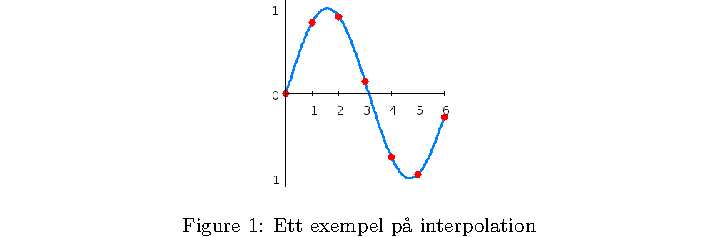
\includegraphics[width=\textwidth,clip=true,trim=80 0 80 0]{ex/4/graphicx.pdf}}
		\end{minipage}
		\caption{Koden till vänster inkluderar filen \cli{interpolation.png} i
		\LaTeX-dokumentet och ger det resultat som ses till höger.}
		\label{fig:graphicx}
	\end{figure}
	
	\subsubsection{Rätt format?}
	En nackdel med \pdfLaTeX{} när det gäller \pack{graphicx} är att det inte
	finns särskilt många bildformat som fungerar (dock fler än för gamla
	\LaTeX{}, som bara accepterade \EPS). De enda format som kan inkluderas
	med \pack{graphicx} när man använder \pdfLaTeX{} är \textsc{PNG},
	\textsc{JPEG} och \PDF. Oftast vill man använda \PDF{} för figurer,
	eftersom
	det är det enda vektorbaserade formatet som fungerar, medan man för
	fotografier och dylikt använder \textsc{JPEG}. \textsc{PNG} kan man
	använda då man egentligen bör använda \PDF{} men detta inte är möjligt.
	
	Eftersom många verktyg och programvaror fortfarande sparar filer i
	\EPS-format kan det vara praktiskt att kunna konvertera dessa till ett
	format som fungerar. Detta kan göras med verktyget \cli{epstopdf}, som
	finns tillgängligt på CTAN.
	
	\subsection{Rita med \PGFTikZ}
	Ett lite mer komplicerat sätt att inkludera grafik (men ofta 
	föredelaktigt, eftersom allt innehåll stannar i \TeX-filen) är att använda
	\PGFTikZ, ett paket skrivet för att användas med \pdfLaTeX{} för att rita
	figurer i \LaTeX{}. Med det kan man direkt i sitt \LaTeX-dokument skapa
	enklare figurer som flödesscheman, träd, grafer eller liknande; se exempel
	i figur~\vref{fig:tikz}. Även mer avancerade figurer är möjliga, men att
	förklara hela \PGFTikZ{} tar allt för lång tid för denna introduktion. Den
	intresserade läsaren hänvisas istället till \citeasnoun{Mertz07} som har
	en bra introduktion till ämnet, och \PGFTikZ-manualen \cite{Tantau10} som
	utförligt beskriver hur paketet fungerar.
	
	\begin{figure}[p]
		\centering
		\begin{minipage}{0.95\textwidth} % kod
			\vfil
			\begin{minted}[frame=single]{latex}
\newcounter{d}\setcounter{d}{0}\def\mcolor{SpringGreen}
\begin{tikzpicture}
    \path[coordinate] (0,0) coordinate(A) ++( 60:6cm)
                      coordinate(B) ++(-60:6cm) coordinate(C);
    \draw[fill=Black!\thed!\mcolor] (A) -- (B) -- (C) -- cycle;
    \foreach \x in {1,...,15}{%
        \pgfmathsetcounter{d}{\thed+10}
        \setcounter{d}{\thed}
        \path[coordinate] coordinate(X) at (A){};
        \path[coordinate] (A) -- (B) coordinate[pos=.15](A)
                            -- (C) coordinate[pos=.15](B)
                            -- (X) coordinate[pos=.15](C);
        \draw[fill=Black!\thed!\mcolor]
				(A)--(B)--(C)--cycle;
    }
\end{tikzpicture}
			\end{minted}
			\vfil
		\end{minipage}
		\\[1ex]
		\begin{minipage}{0.95\textwidth} % figur
			\centering
			\newcounter{density}\setcounter{density}{0}
			\begin{minipage}{0.475\textwidth}
			\fbox{\begin{tikzpicture}
			    \path[coordinate] (0,0)  coordinate(A)
			                ++( 60:6cm) coordinate(B)
			                ++(-60:6cm) coordinate(C);
			    \draw[fill=Black!\thedensity!SpringGreen]
							(A) -- (B) -- (C) -- cycle;
			    \foreach \x in {1,...,15}{%
			        \pgfmathsetcounter{density}{\thedensity+10}
			        \setcounter{density}{\thedensity}
			        \path[coordinate] coordinate(X) at (A){};
			        \path[coordinate] (A) -- (B) coordinate[pos=.15](A)
			                            -- (C) coordinate[pos=.15](B)
			                            -- (X) coordinate[pos=.15](C);
			        \draw[fill=Black!\thedensity!SpringGreen]
							(A)--(B)--(C)--cycle;
			    }
			\end{tikzpicture}}
			\end{minipage}\hfil
			\begin{minipage}{0.475\textwidth}
			\caption[Koden ovan tolkas av \PGFTikZ{} och resulterar i den
			itererade triangeln till vänster]{
			Koden ovan tolkas av \PGFTikZ{} och resulterar i den
			itererade triangeln till vänster.
			Fler exempel finns i
			\citeasnoun{Mertz07} och \citeasnoun{Tantau10}. Tack till Alain 
			Matthes för originalkoden\footnote{\url{http://www.texample.net/tikz/examples/rotated-triangle/}}.}
			\label{fig:tikz}
			\end{minipage}
		\end{minipage}
	\end{figure}
	
	\label{sec:4:end}
	%% (end)
	
	%% REFERENSER MED BIBTEX (fold)
	\section{Referenser med \BibTeX}\label{sec:5}
	%% (end)
	
	%% VIDARE LÄSNING (fold)
	\section{Vidare läsning}\label{sec:6}
	
	\subsection{Andra resurser}
	\subsubsection{Böcker och artiklar}
	\subsubsection{Hjälp med specifika problem}
	% TeX.SE!
	
	\subsection{Rekommenderade paket}
	
	\subsection{Tips för stora projekt}
	
	\subsection{Andra \TeX-baserade projekt}
	\subsubsection{Unicode-baserade \XeTeX}
	\subsubsection{Skripta med \hologo{LuaTeX}}
	%% (end)
	
	\let\oldurl=\url\renewcommand\url[1]{\newline{\small\oldurl{#1}}}
	\bibliography{referenser}
	\addcontentsline{toc}{section}{\hspace{1.3em}Referenser}
	
	\appendix
	%% EN ENKEL MALL (fold)
	\section{En enkel mall}\label{app:1}
	
	%% (end)

	\backmatter 
	\pagestyle{empty}
	\cleardoublepage\hbox{}\newpage
	{ % EXTERNAL BACK PAGE (fold)
		\pagecolor{\frontpagecolor}
		\color{White}
		\frontpagegraphic
		\begin{tikzpicture}[remember picture,overlay]
			\node [anchor=south east,above=2cm,right=-3.75cm] at (current page.south east)
			 			{
\includegraphics[width=3cm]{qrcode.pdf}};
		\end{tikzpicture}
		\normalcolor
		\newpage
		\pagecolor{White}
	} % (end)
\end{document}